\documentclass{beamer}
\usepackage{listings}
\usepackage{mdframed}
\usepackage{tikz}
\usepackage{pdfpages}
\usepackage{amssymb}% http://ctan.org/pkg/amssymb
\usepackage{pifont}% http://ctan.org/pkg/pifont
\usepackage[overlay,absolute]{textpos}

\usepackage[francais]{babel}
\usepackage[utf8]{inputenc}

\usepackage{float}
\usepackage{graphicx}
\usepackage{wrapfig}
\usepackage{times}
\usepackage[T1]{fontenc}

\makeatletter
\hypersetup{pdfpagemode=FullScreen}

\newcommand{\firstlogo}{images/ups.jpg}
\newcommand{\secondlogo}{images/Toulouse.png}
\newcommand{\footsubject}{Architecture multi-couches et développement avec Java EE} % Subject in footer
\newcommand{\cmark}{\ding{51}}%
\newcommand{\xmark}{\ding{55}}%

\newcommand{\rgbcolortheme}{119,30,72}

\mode<presentation> {
	\usepackage{../beamer-theme/beamerthemeUNLTheme}
}

\title[] % Not required. If title is too long 
{Toulouse Musée}
\subtitle{Architecture multi-couches et développement avec Java EE}

\newcommand{\authors}{%
Antoine de \bsc{Roquemaurel}\newline Florent \bsc{Berbie}
}

\newcommand{\FlorentSpeak}{%
\author[
\textbf{\color{white} F}lorent\\
{A}ntoine
]{\authors}
}

\newcommand{\AntoineSpeak}{%
\author[
{F}lorent\\
\textbf{\color{white} A}ntoine
]{\authors}
}

\newcommand{\NoOneSpeak}{%%
\author[
Florent\\
Antoine
]{\authors}
}


\institute[] 
{
  Universit\'e Toulouse III -- Paul Sabatier \\
  M1 Informatique -- Développement Logiciel 
  \vspace{-10px}
}
\date[ ~ ~ ~ 27 / 04 / 2015] % In footer 
{Lundi 27 Avril 2015}


 % Toc for each section
\AtBeginSection[] {
  \begin{frame}<beamer>{Ligne directrice}
    \tableofcontents[currentsection]
  \end{frame}
}

\NoOneSpeak
\begin{document}
	\sidetoc{no}
	\begin{frame}
		\titlepage
	\end{frame}
	\FlorentSpeak
\begin{frame}{Objectifs du projet : bla bla} % TODO	
\end{frame}

	\begin{frame}
		\tableofcontents
	\end{frame}
	\sidetoc{yes}
	\section{Organisation du travail} % TODO
	\AntoineSpeak	
\subsection{Github  et travail collaboratif}	% A Florent
\begin{frame}{Github, plateforme de travail collaboratif} % A.  
	\begin{itemize}
		\item Communication et versionnement
		\begin{figure}
			\centering
			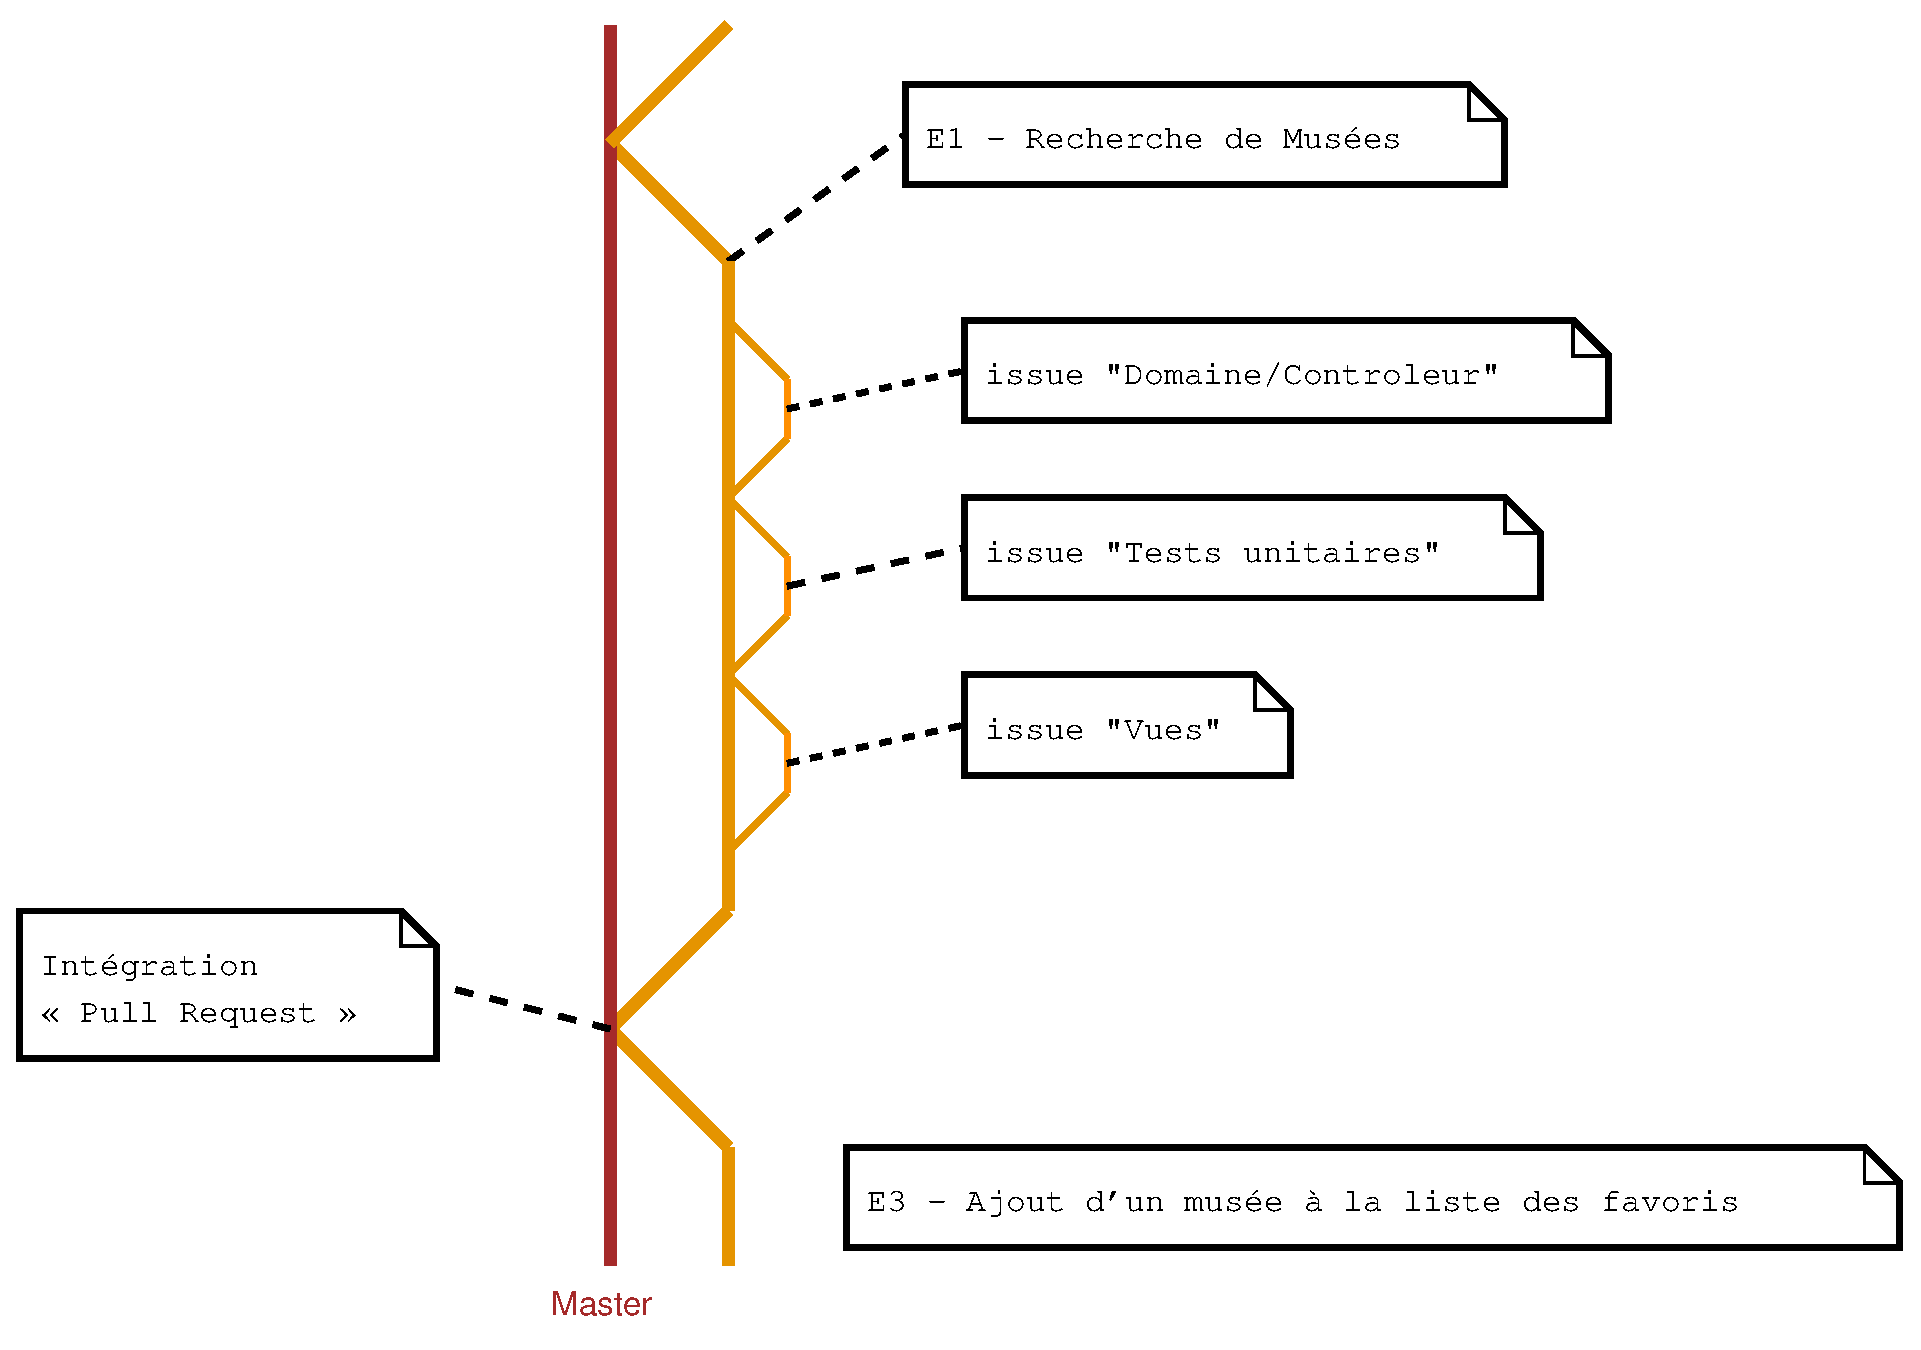
\includegraphics[width=9cm]{./images/workflow_github}
			\caption{Workflow sur GitHub}
			\label{fig:workflow_github}
		\end{figure}
	\end{itemize}
\end{frame}

\begin{frame}{Github, plateforme de travail collaboratif} % A.
	\begin{block}{Une exigence est terminée, si}
		\begin{itemize}
			\item Le code est \textbf{lisible} et \textbf{compréhensible}
			\item Le code est correctement \textbf{documenté}
			\item Les \textbf{tests} passent \cmark
		\end{itemize} 
	\end{block}
	\pause

	\begin{block}{Utilisation des Pull Requests}
		\begin{itemize}
			\item Création par la personne s'affectant l'issue
			\item Description du travail accompli
			\item PR validée par un autre membre de l'équipe
				\begin{itemize}
					\item Respect de la définition de \textbf{<< finie >>}
					\item \textbf{Tests fonctionnels} \cmark
				\end{itemize}
		\end{itemize}
	\end{block}
\end{frame}


	\FlorentSpeak
\subsection{Le Pair-Programming}
\begin{frame}{Le Pair-Programming}
	\pause
	\begin{exampleblock}{Des avantages…}
		\begin{itemize}
			\item Code plus \textbf{propre}, plus \textbf{compréhensible}
			\item Résolution des problèmes plus rapidement
			\item Moins de bugs
			\item Particulièrement \textbf{adapté à ce projet}!
		\end{itemize}
\end{exampleblock}
	\pause
\vfill
\begin{alertblock}{Et des inconvénients}
\begin{itemize}
	\item Développement plus lent au sein d'une \textit{User Story}
\end{itemize}
\end{alertblock}
\end{frame}
	

	\section{Conception de l'application} % TODO
	\AntoineSpeak
\subsection{Domaine métier}
\begin{frame}{Domaines métier}
	\begin{figure}
		\centering
		%\only<1>{
		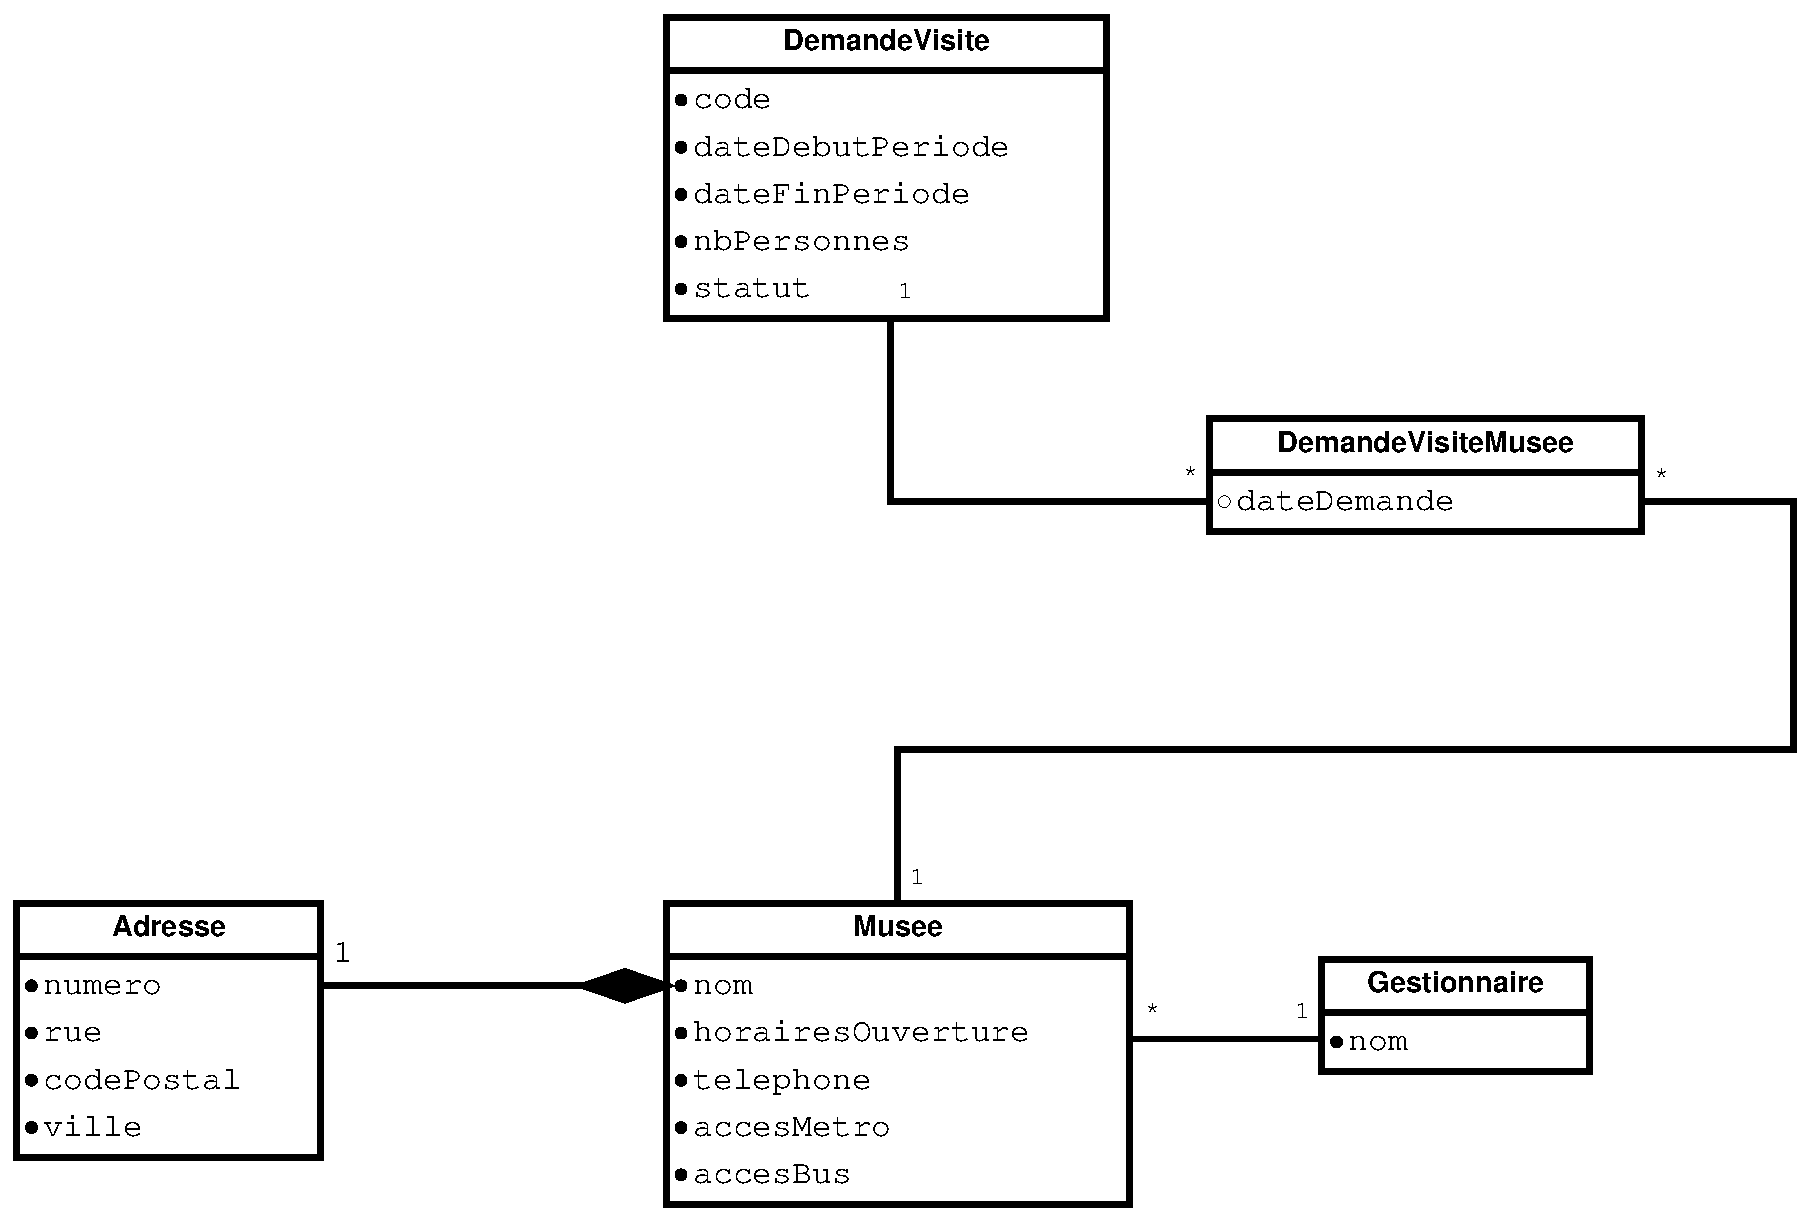
\includegraphics[width=9.75cm]{images/new_database.eps}
		\caption{Domaine métier}
		%}		
	\end{figure}
\end{frame}

	\FlorentSpeak
\subsection{Services}
\begin{frame}{Services}
	\pause
	\begin{block}{Musées}
		\begin{itemize}
			\item Recherche des musées (Nom, Code Postal, Rue)
			\item Transactionnel
		\end{itemize}
	\end{block}	
	\vfill
	\pause
	\begin{block}{$\bigstar$ Favoris}
		\begin{itemize}
			\item Gestion des musées favoris
			\begin{itemize}
				\item Ajouter aux favoris
				\item Retirer des favoris
			\end{itemize}
			\item Gestion des favoris par session
		\end{itemize}
	\end{block}
	\pause
	\vfill	
	\begin{block}{Demande de visite}
		\begin{itemize}
			\item Effectuer une demande de visite				
			\item Stocké en base de données
		\end{itemize}
	\end{block}
\end{frame}
	\subsection{Qualit\'e du code}
	\section{Résultats} % TODO	
	\AntoineSpeak
\subsection{Recherche des mus\'ees}
\begin{frame}{Musées favoris et demande de visite}
	\begin{figure}
		\centering
		\only<1>{
		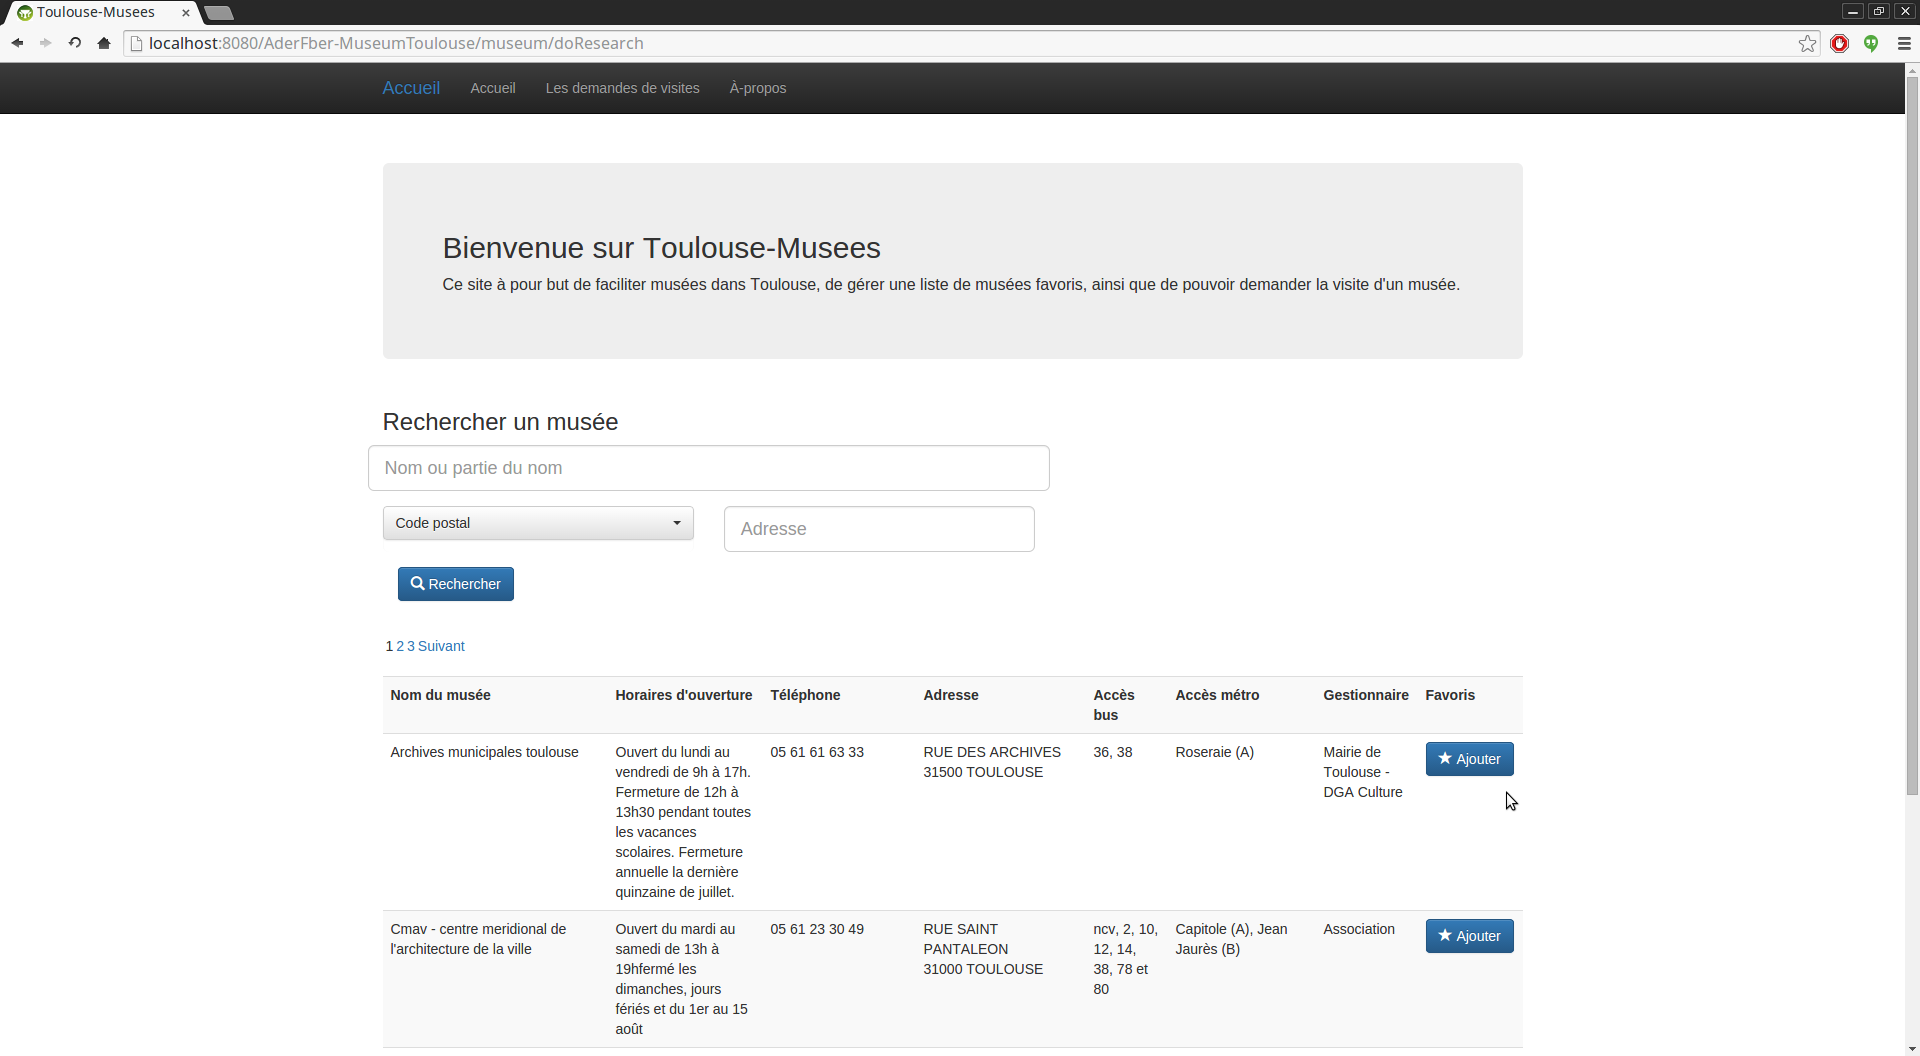
\includegraphics[width=8.5cm]{screens/accueil_with_museums.png}
		\caption{Liste des musées}
		}
		
		\only<2> { 
		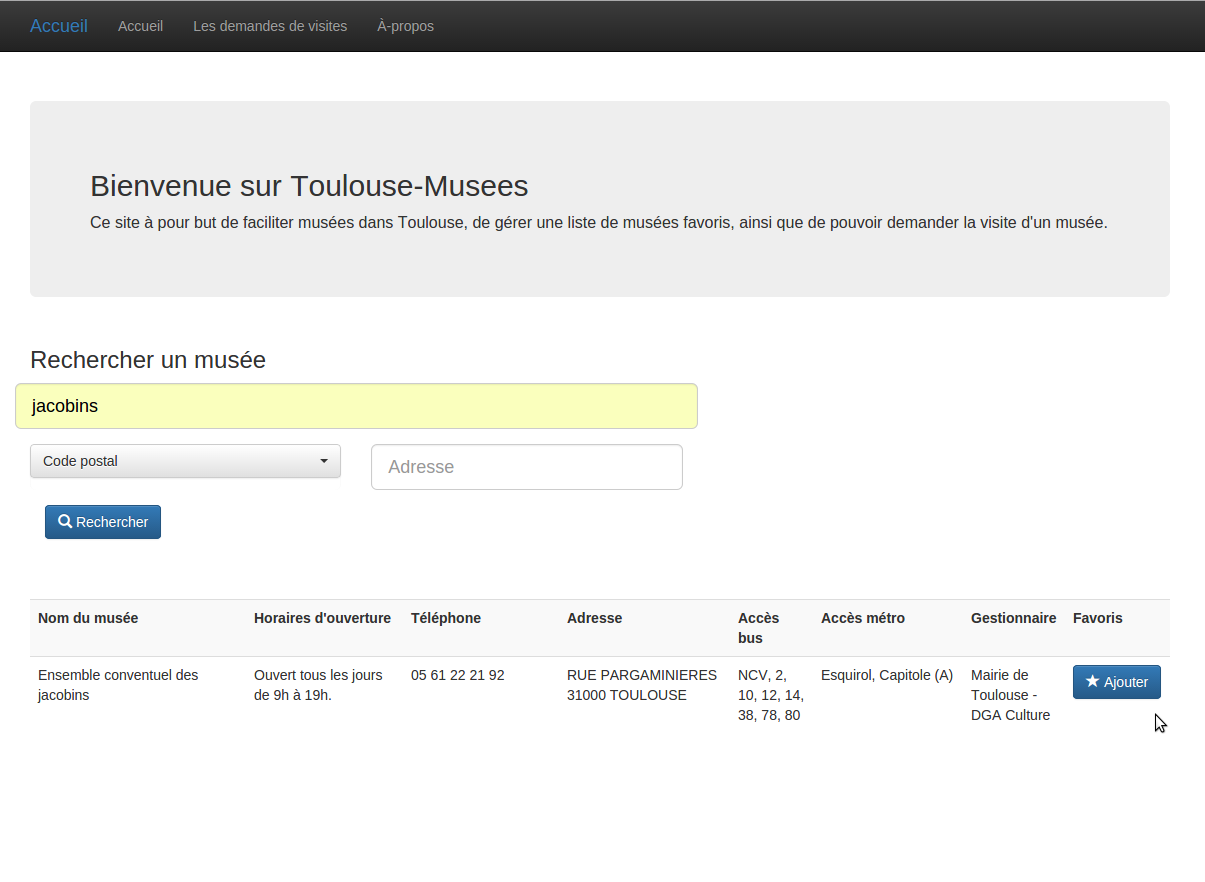
\includegraphics[width=9.25cm]{screens/search_by_name.png}
		\caption{Recherche des musées par nom}
		}

		\only<3> { 
		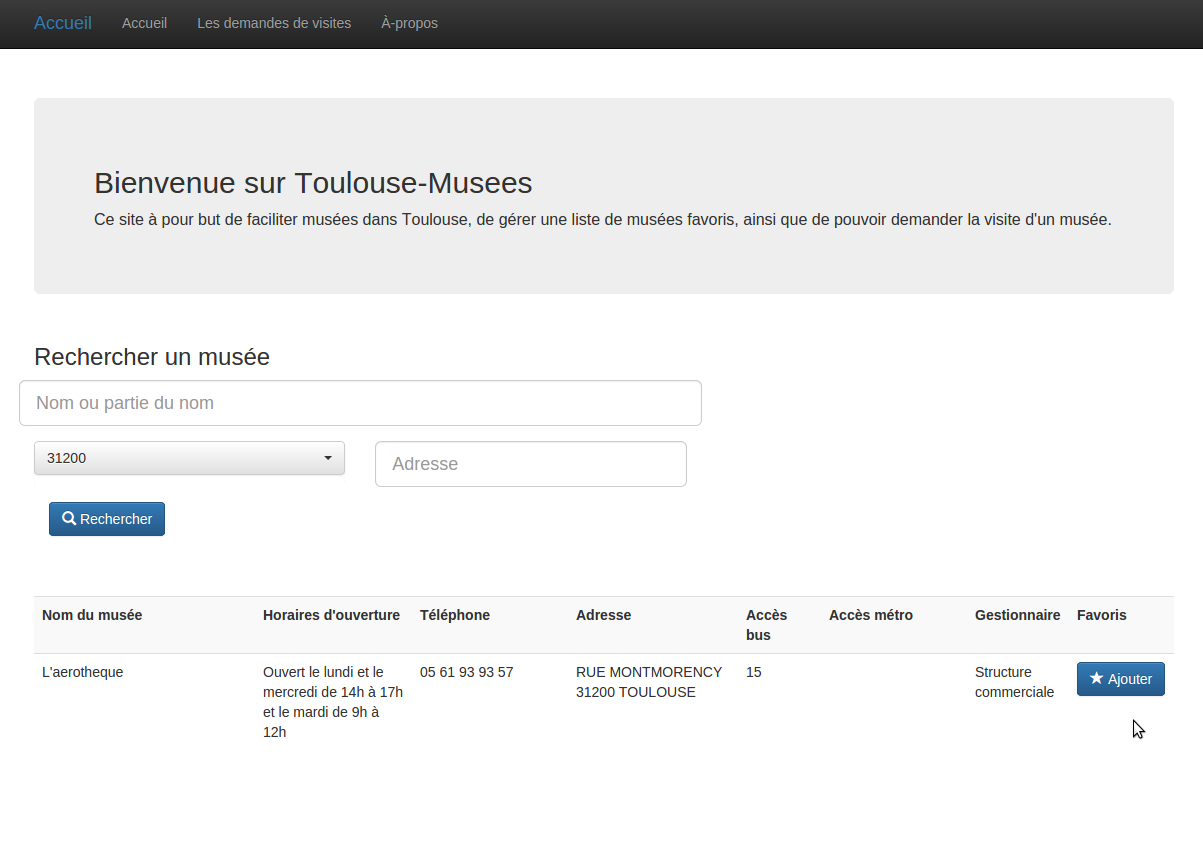
\includegraphics[width=9cm]{screens/search_by_postalcode.png}
		\caption{Recherche des musées par Code postal}
		}
		
		\only<4> { 
		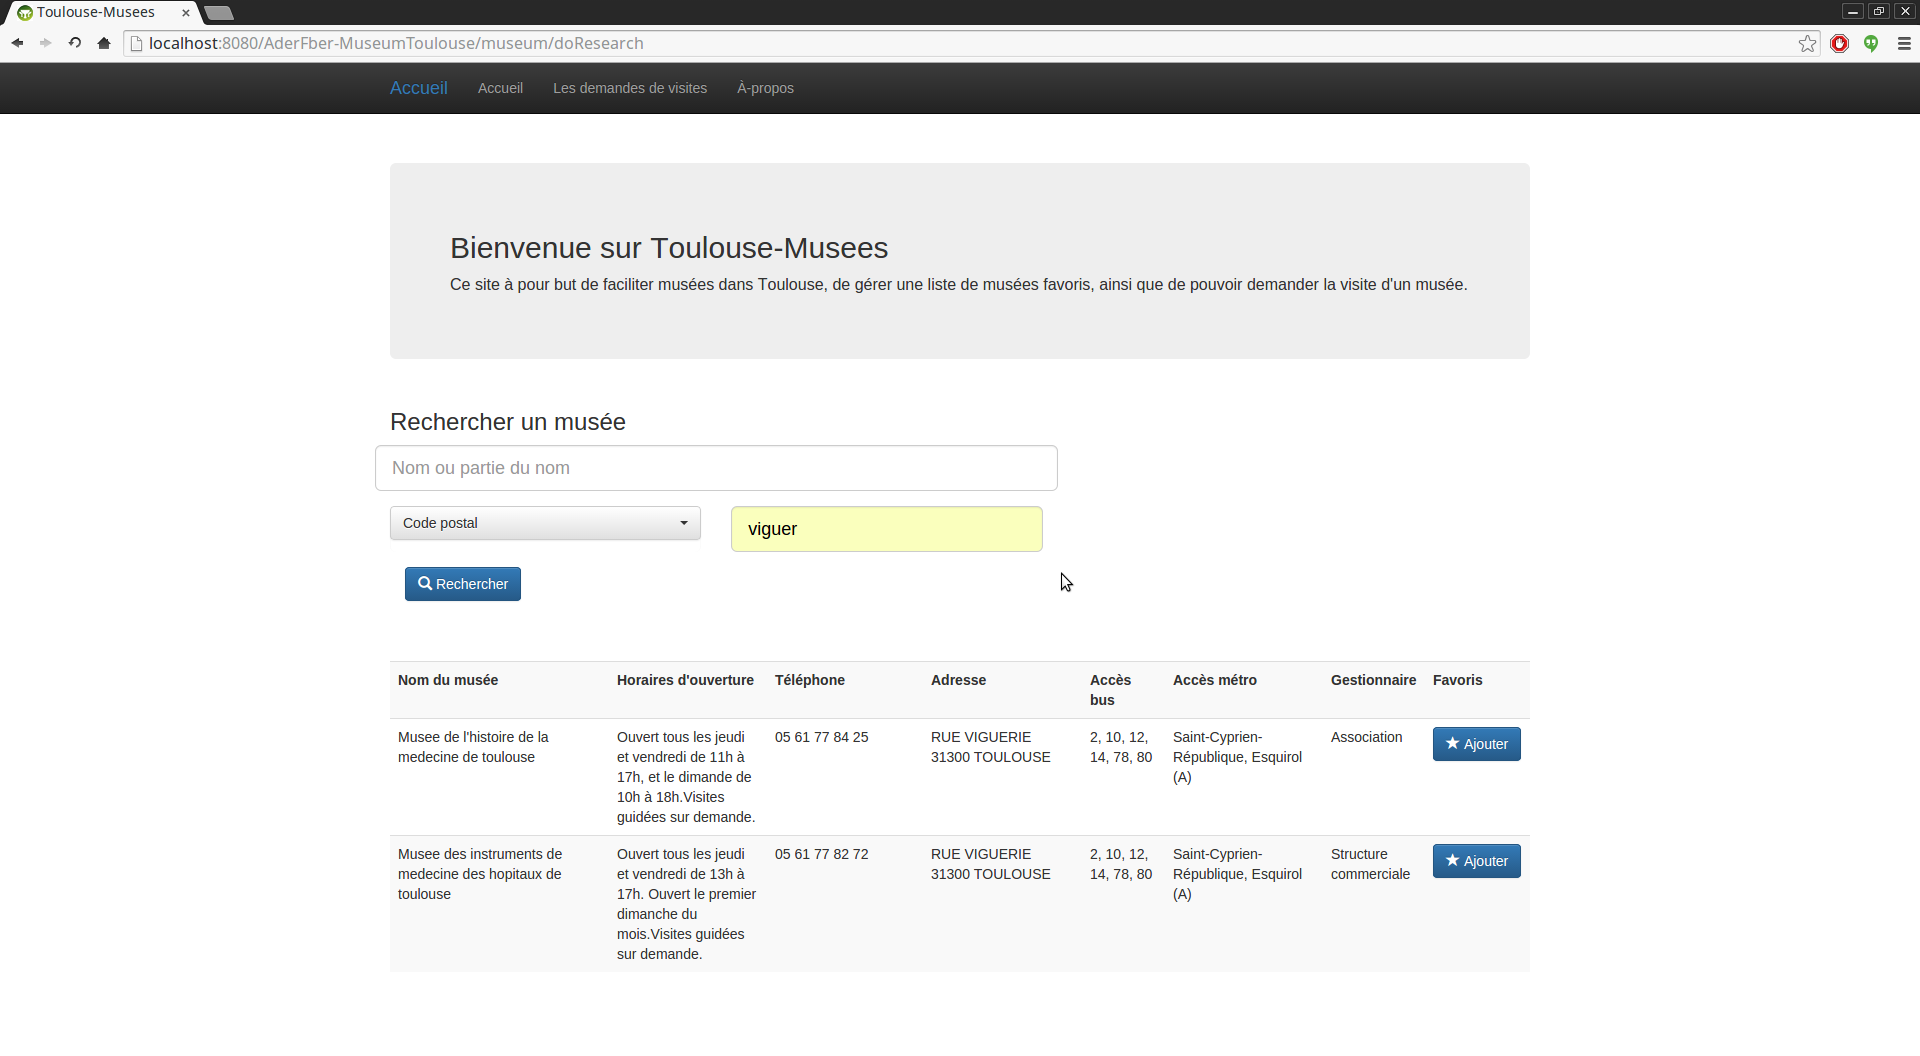
\includegraphics[width=9cm]{screens/search_by_address.png}
		\caption{Recherche des musées par nom de rue}
		}
		
		
		
	\end{figure}
\end{frame}
	\AntoineSpeak
\subsection{Mus\'es favoris et demande de visite}
	\section{}
	\AntoineSpeak
\begin{frame}{Conclusion}
	\pause
	\begin{alertblock}{Les moins}
		\begin{itemize}
			\item Temps d'adaptation à \textit{Grails}
			% \item Tests fonctionnels valide en foncton de la machine ?
		\end{itemize}
	\end{alertblock}
	\pause
	\vfill
	\begin{exampleblock}{Les plus}
		\begin{itemize}
			\item Ensemble des exigences  \cmark
			\item Expérience technique
			\item Expérience en travail collaboratif
		\end{itemize}
	\end{exampleblock}	
\end{frame}


	\sidetoc{no}
	\NoOneSpeak
	\begin{frame}{Avez-vous des questions ?}
		\begin{figure}[H]
			\centering
			
\includegraphics[width=5cm]{questions.png}
		\end{figure}
	\end{frame}
\end{document}
